%%%%%%%%%%%%%%%%%%%%% chapter.tex %%%%%%%%%%%%%%%%%%%%%%%%%%%%%%%%%
%
% sample chapter
%
% Use this file as a template for your own input.
%
%%%%%%%%%%%%%%%%%%%%%%%% Springer-Verlag %%%%%%%%%%%%%%%%%%%%%%%%%%
%\motto{Use the template \emph{chapter.tex} to style the various elements of your chapter content.}
\chapter{Elements of Special Relativity}
\label{Relativity} % Always give \ unique label
% use \chaptermark{}
% to alter or adjust the chapter heading in the running 
\begin{postulate}[Galileian Relativity]
\label{postulate:galileian-relativity}
The laws of mechanics are the same in all inertial reference frames.\\
\end{postulate}
Inertial Reference Frame: a reference frame in which the 1st law of motion holds exactly (a point-like body without forces acting on it either is still or is moving with constant velocity)

As an immediate consequence, in an inertial reference frame it's impossible to determine if the frame itself is moving. 
\begin{figure}
    \centering
    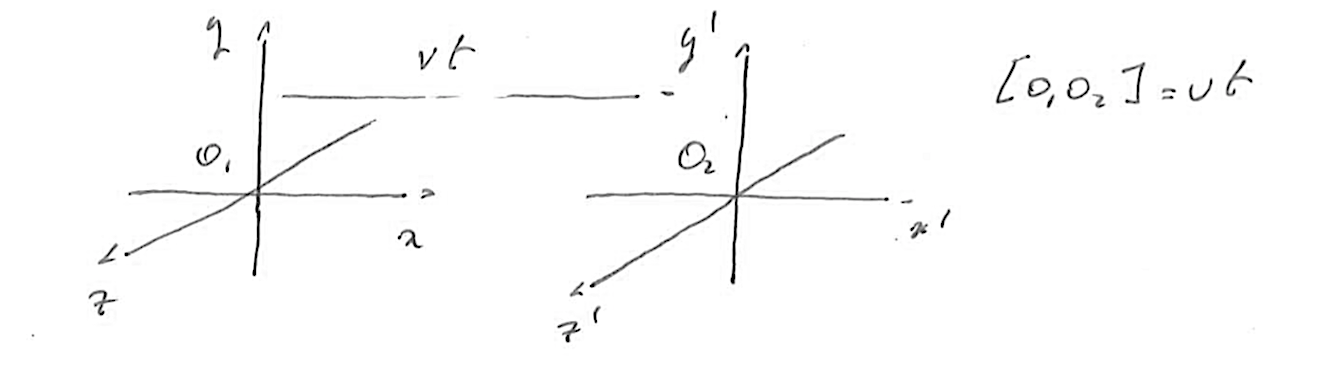
\includegraphics[width=\textwidth]{rel1}
    \caption{An example of an inertial $\mathcal{O}'$ frame moving with respect to another inertial frame $\mathcal{O}$ at constant velocity $v$.}
    \label{fig:rel1}
\end{figure}
A Galilean Transformation allows to determine the relation between the coordinates of two inertial reference frames. With reference to figure \ref{fig:rel1} the relations are the following:

\begin{equation}
\begin{cases}
&x = x' + vt\\
&y = y'\\
&z = z'\\
&t = t'\\  
\end{cases}
\hspace{2cm}
\begin{cases}
x' = x' - vt\\
y' = y'\\
z' = z\\
t = t'\\  
\end{cases}
\end{equation}

The fundamental point in these equations is that the coordinate changes only along the directions for which $\vec{v}\div0$.\\

The diverging point from Galileian Relativity is an immediate consequence of Maxwell's equations, in fact, it can be easily proven that the assuming Maxwell's equation validity implies that electromagnetic waves are moving at a constant velocity $c$
\[c\simeq3\times10^8 \meter / \second\]

At the time of the discovery of Maxwell's equations, physicists were not comfortable with the idea that light, and in general electromagnetic waves, are moving through in the void. The common idea at the time was that the light is moving through an invisible medium, which is uniformly distributed across the Universe: the \emph{Eather}.


\section{Introduction and the Michelson Morley Experiment}
In order to verify the existence of the Eather, Michelson and Morley developed a particularly sensible experiment, which layout is shown in figure \ref{fig:rel2}

\begin{figure}
    \centering
    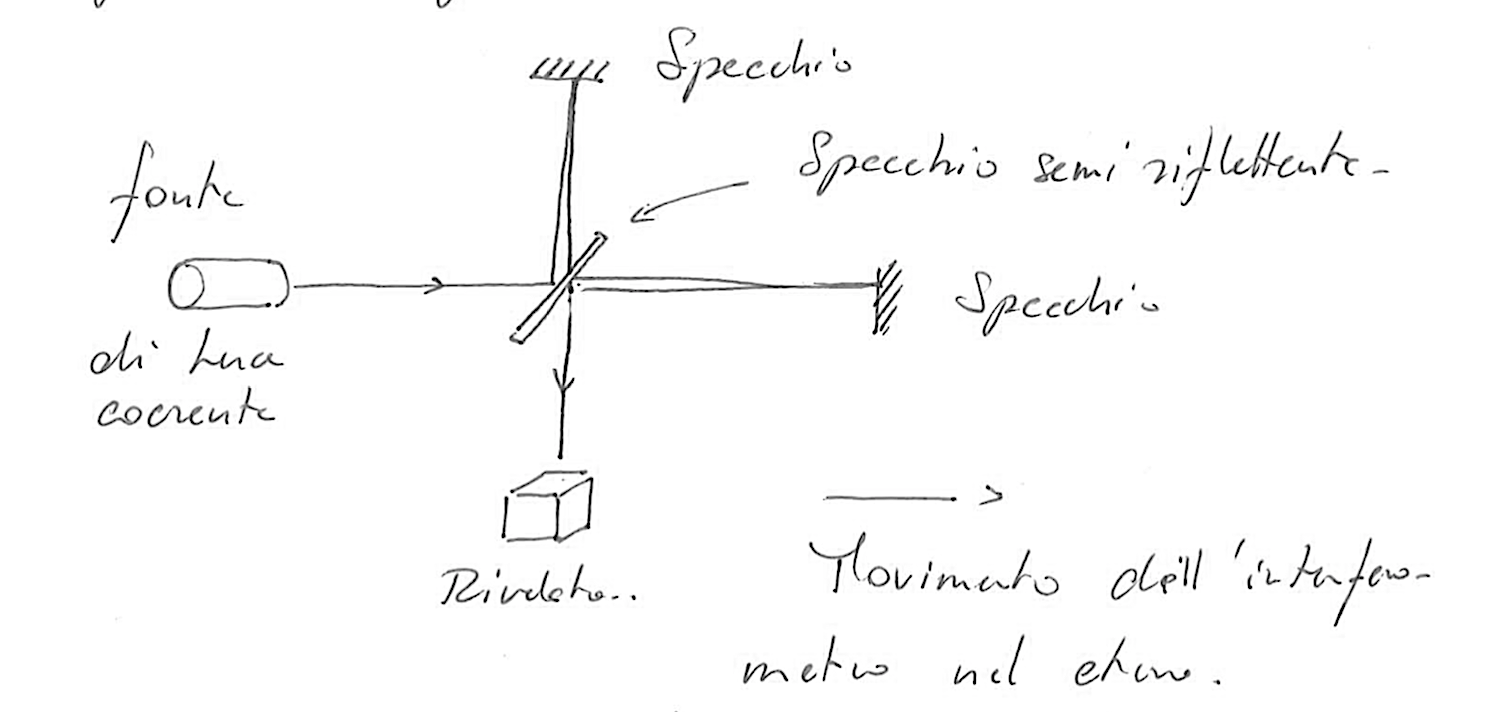
\includegraphics[width=0.8\textwidth]{rel2}
    \caption{Caption}
    \label{fig:rel2}
\end{figure}{}


If the interferometer is moving through the Eather, then the light (which is moving at $c$ with reference to the Eather) will travel the distance of the two arms of the spectrometer in a different time, then a corresponding interference figure will be produced between the two beams.\\

No such interference was visible with the Michelson and Morley experiment, only after that physicists started to reject the idea of the Eather, and accept the fact that light travels at the same speed in all reference frames.





\section{From Simultaneity to Lorentz Transforms}
The theory of \emph{Special Relativity} is the theory which aims to describe space (and time) transformation between two inertial reference frames, one of which is moving with a constant velocity $\vec{v}$ with respect to the other.\\

The foundation of Special Relativity is on the following postulate, which is considered in addition to Postulate \ref{postulate:galileian-relativity}.

\begin{postulate}[Invariance of $c$]
\label{postulate:invariance-of-c}
The speed of light $c$ has the same value in all inertial reference frames. Its value is equal to
\[c = 299792458 \meter/\second\]
\end{postulate}

The theory of Special Relativity was built by Albert Einstein, starting from these two postulates, and exploiting more deeply the concept of \emph{Simultaneity}.
Einstein's definition of simultaneity follows from this example, consider two events which happen in two different points of the coordinate space, if each one o them emit a light beam directed to the other event's position, then if an observer which is in the middle of them see both the light beams at the same time the two events can be considered simultaneous.\\

\begin{figure}
    \centering
    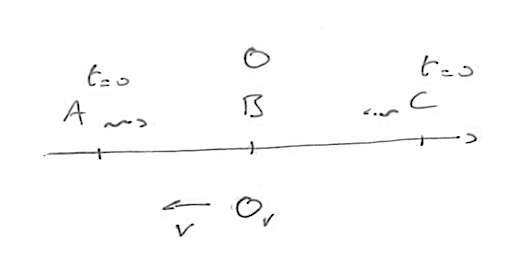
\includegraphics[width=0.8\textwidth]{rel3}
    \label{fig:rel3}
\end{figure}{}

Let's make a more detailed overview of this example. With reference to figure \ref{fig:rel3}, an observer $O$ which is in $B$, fixed with respect to $A$ and $C$m  will see the light from $A$ and $C$ simultaneously. Instead an observer $O'$ which is moving with constant velocity $\vec{v}$ will see the light from $A$ before the light coming from $C$. In general, we have to take into account the fact that simultaneity depends on the reference frame!\\

We can consider the example in the reference frame of $O'$ with the coordinatex $(x,t)$, as in figure \ref{fig:rel4}. 

\begin{figure}
    \centering
    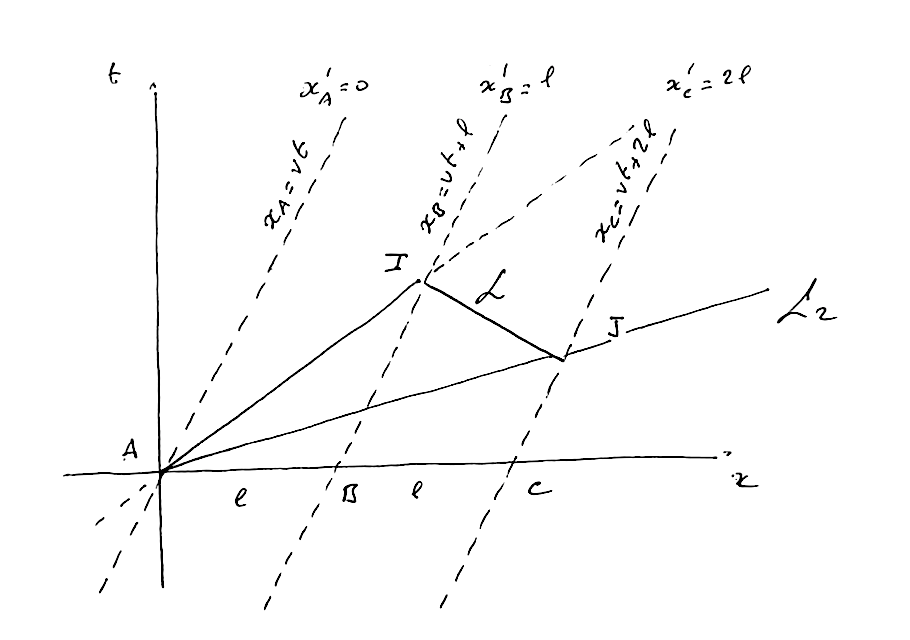
\includegraphics[width=0.8\textwidth]{rel4}
    \label{fig:rel4}
    \caption{In this figure, the coordinates (x,t) belong to the reference frame of $O'$, which is moving at constant velocity $\vec{v}$ with respect to the points $A$, $B$ and $C$. Coordinates $(x',t')$ are the coordinates of the observer $O$, fixed with respect to $A$, $B$ and $C$.}
\end{figure}{}


Let us compute the coordinates of the event ``Beam from A arrives in B'': $(x_I,t_I)$.

\[x_I=vt_I+l\]
\[x_I=ct_I\]
\[vt_I+l=ct_I\]
which leads us to

\begin{equation}
t_I=\frac{l}{c-v} \hfill x_I=\frac{cl}{c-v}
\end{equation}

Now let's compute the equation of the line $L$.
\[L:\ \ x=ct+\alpha\]
Point $I$ satisfies the equation, so
\[\frac{cl}{c-v} = \frac{cl}{c-v} + \alpha\]
\[\alpha = \frac{2cl}{c-v} = \frac{2l}{1-\frac{v}{c}}\]
and denoting
\begin{equation}
  \label{eq:beta}
  beta = \frac{v}{c}
\end{equation}

we finally obtain
\begin{equation}
  L:\ \ x=ct+\frac{2l}{1-\beta}
\end{equation}

The coordinate of $J$ are then:
\begin{eqnarray*}
  x_J = vt_J+2l &=& ct_J+\frac{2l}{1-\beta}\\
  \left[v+c\right]t-J &=& 2l \left[\frac{1}{1-\beta}-1\right]\\
  c\left[1+\beta\right]t-J &=& 2l \left[\frac{1-1+\beta}{1-\beta}\right]\\
  \left[1+\beta\right]t-J &=& \frac{2l}{c} \left[\frac{\beta}{1-\beta}\right]\\
\end{eqnarray*}
which gives us
\begin{equation}
  t_J =\frac{2l}{c}\,\frac{1}{1-\beta^2}
\end{equation}
and
\begin{eqnarray*}
  x_J &=& vt_J+2l\\
  &=& 2l \frac{\beta^2}{1-\beta^2} + 2l\,\frac{1-\beta^2}{1-\beta^2}\\
  &=& 2l \frac{1}{1-\beta^2}
\end{eqnarray*}
\begin{equation}
  x_J = \frac{c}{\beta}\,t_J
\end{equation}

which is also the equation for the line $L_2$. Each point on $L_2$ corresponds to simultaneous event.\\

It's important to search now the correct transformation which allows us to go from the coordinates $(x,t)$ to $(x',t')$. If $x = vt $ then the coordinate $x'$ should be zero. This implies that
\[x' = f(v)\cdot(x-vt)\]
For the same reason, we get that for $t'=0$ whenever $t = xv/c^2 $, so the following funcional form is expected for $t'$:
\[t' = g(v)\cdot\left(t-\frac{v}{c^2}x\right)\]

Let's now consider the condition that $c$ is constant and its value is equal for any reference frame. Then the following condition must hold:
\begin{equation}
\label{eq:B:1}
  \begin{cases}
    x = ct\\
    x'=ct'\\
  \end{cases}
\end{equation}

\begin{eqnarray*}
  x' &= (x-vt)\cdot f(v) = (ct-vt)\cdot f(v)\\
  &= t(c-v)\cdot f(v)\\
  t' &= \left(t-\frac{v}{c}t\right)\cdot g(v)\\
  &= \frac{1}{c} (c-v) t \cdot g(v)\\
  &= \frac{1}{c} x' \frac{g(v)}{f(v)}
\end{eqnarray*}
Then equation \ref{eq:B:1} is satisfied if and only if:
\[g(v) = f(v)\]

If the laws of physics are invariant in any inertial reference frame, then there's no difference in considering the expression of coordinates $(x',t')$ as function of $(x,t)$ or \emph{vice versa}. The expression of $(x,t)$ as function of $(x',t')$ should have the same functional form, but with an opposite velocity term:

\begin{equation}
  \begin{cases}
    x = (x'+vt')f(v)\\
    t = \left(t' + \frac{v}{c^2}x\right)f(v)
    \end{cases}
\end{equation}

\begin{eqnarray*}
  x &=& \left[ \left( x-vt\right)f(v)+\left(vt-\beta^2x\right)f(v)\right]f(v)\\
  &=& x\left[f(v)^2\left(1-\beta^2\right)\right]
\end{eqnarray*}
this leads us to the definition of
\begin{equation}
  \label{eq:gamma}
\gamma = f(v) = \frac{1}{\sqrt{1-\beta^2}}
\end{equation}

and the expression of Lorentz' transformations:

\begin{eqnarray}
  x' &=& \frac{x-vt}{\sqrt{1-\frac{v^2}{c^2}}}\\
  t' &=& \frac{t-\frac{v}{c^2}x}{\sqrt{1-\frac{v^2}{c^2}}}\\
\end{eqnarray}

Note that in the limit of $v/c << 1$ the Galileian expression of coordinate transformations is recovered. If we consider a Lorentz' transformation in three dimensions we could always make a rotation of the reference frame which bring our coordinate system with an axis ($x$ for example) parallel to $\vec{v}$. Then coordinates which belongs to the axes which are ortogonal to the motion direction will not be affected by the transformation. The following is the expression of the Lorentz' transformation making explicit use of \ref{eq:beta} and \ref{eq:gamma}:
\begin{eqnarray}
  x' &=& \gamma x -\beta\gamma c t \\
  ct' &=& \gamma ct -\beta\gamma x
\end{eqnarray}

RIPRENDI DA PAG 8 LATO DESTRO
\section{Lorentz invariants} 
\section{Relativistic Action of a Particle and Hamiltonian}
\section{Covariant Notations}

